\section{Client-server architecture}

\begin{figure}[H]
    \centering
    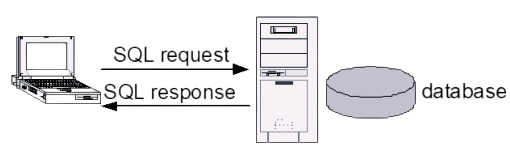
\includegraphics[width=0.4\linewidth]{images/cs.png}
    \caption{Client-server architecture}
\end{figure}
The hardware used by this the client-server architecture is: 
\begin{itemize}
    \item Server for data management. 
    \item Client for presentation layout. 
\end{itemize}
The software used by this type of architecture is: 
\begin{itemize}
    \item Client software sends requests to the server by means of SQL queries. The software in the client contains both business and presentation logic. 
    \item Server software processes the query and responds sending the result set back to the client. The software in the server deals with data. 
\end{itemize}
The network topology is based on a local are network with one or more servers and $N$ clients. 